\documentclass[letterpaper,10pt,twoside,twocolumn,openany]{book}
\usepackage[english]{babel}
\usepackage[bg=full,layout=true]{dnd}
\usepackage{graphicx}
\graphicspath{ {./assets/} {../assets/} }
\usepackage{dndnotes}
\usepackage{wallpaper}
\usepackage{subfiles}
\usepackage[utf8]{inputenc}
\usepackage[T1]{fontenc}
\usepackage{textcomp}
\usepackage{amsmath, amssymb}
\usepackage{datetime}
\usepackage{syntax}
% figure support
\usepackage{import}
\usepackage{xifthen}
\usepackage{pdfpages}
\usepackage{transparent}
\newcommand{\incfig}[1]{%
  \def\svgwidth{\columnwidth}
  \import{./figures/}{#1.pdf_tex}
}

\pdfsuppresswarningpagegroup=1

\makeatletter
\global\let\tikz@ensure@dollar@catcode=\relax
\makeatother

\setcounter{tocdepth}{2}

\begin{document}
\frontmatter                           
\begin{titlepage}
  \begin{tikzpicture}[remember picture,overlay]
    \node[inner sep=0pt] at (current page.center) {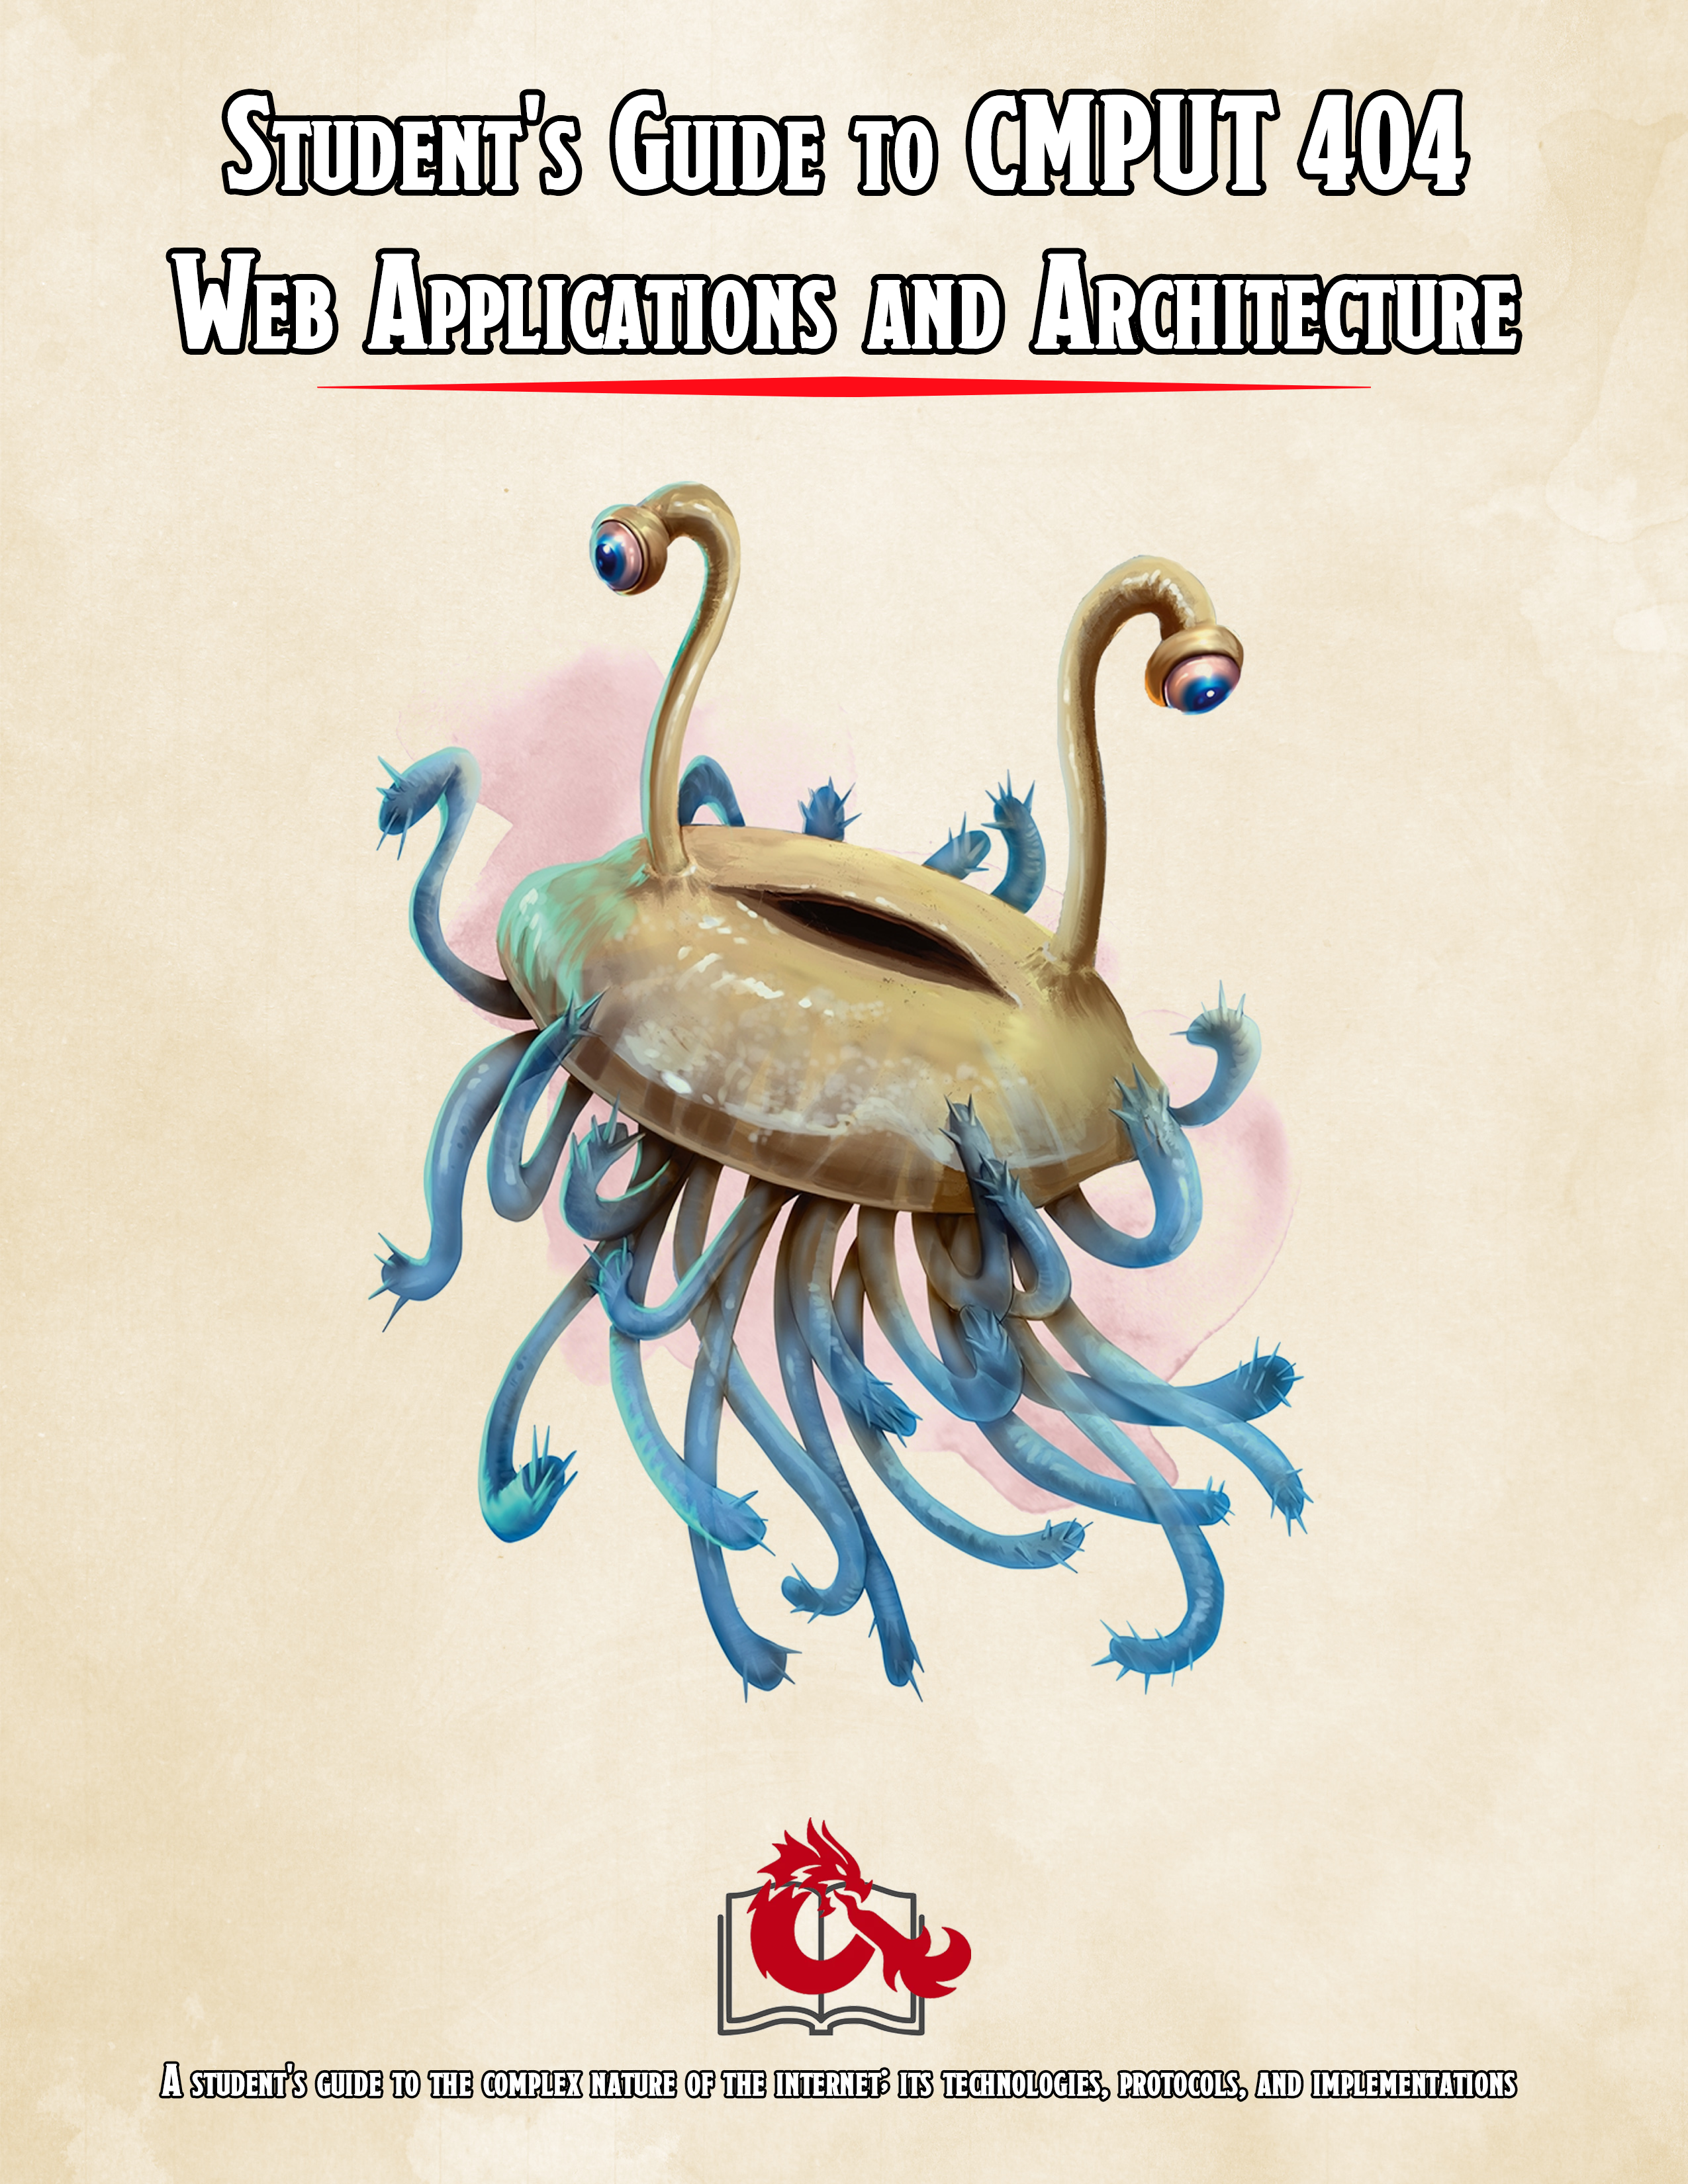
\includegraphics[width=\paperwidth,height=\paperheight]{./CMPUT-404-cover-1.png}};
  \end{tikzpicture}~
  \newpage
  
  \begin{center}


    \large
    \vspace*{\fill}
    Introduction to modern web architecture, from user-facing applications to machine-facing web-services. Topics include: the evolution of the Internet, relevant technologies and protocols, the architecture of modern web-based information systems, web data exchange and serialization, and service-oriented middleware. 
    \\~\\
    By slaying his assignment minions, defeating his midterm champion(s) and ending the final themselves. The heroic legacy of your achievement will be remembered on your academic transcript.
    \\~\\
    \vspace*{\fill}

  \end{center}
  \let\thefootnote\relax\footnote{Disclaimer: This guide is not responsible for the unintentional consequences of GETing the plane of Pandemonium, DELETEing the plane of Elysium, POSTing evil creatures in Mount Celestia, and PUTing Tiamat in the Beastlands.}
\end{titlepage}
\tableofcontents
\mainmatter
\subfile{chapters/chapter2.tex}  
\subfile{chapters/chapter3.tex}  
\subfile{chapters/chapter4.tex}  
\subfile{chapters/chapter5.tex}  
\subfile{chapters/chapter6.tex}  
\subfile{chapters/chapter7.tex}  
\subfile{chapters/chapter8.tex}  
\subfile{chapters/chapter9.tex}  
\subfile{chapters/chapter10.tex} 
\subfile{chapters/chapter11.tex} 
\subfile{chapters/chapter12.tex} 
\subfile{chapters/chapter13.tex} 
\subfile{chapters/chapter14.tex} 
\subfile{chapters/chapter15.tex}
\subfile{chapters/eval.tex}  
\subfile{credit.tex}  
\end{document}
